%%%%%%%%新版本%%%%%%%%%%%%%%%%
\section{Method}
\label{sec:method}

\subsection{Problem: Privilege-Induced Style Drift}
\label{sec:drift}

\begin{wrapfigure}{r}{0.42\linewidth}
  \vspace{-15pt}
  \centering
  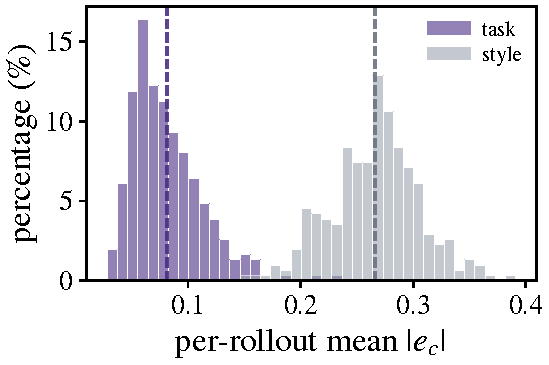
\includegraphics[width=\linewidth]{figs/hist_ec_task_vs_style_singlepair.pdf}
  \caption{Per-rollout mean $|e_{c,t}|$ on style vs.\ task tokens. The
  privilege shifts most of its influence onto style tokens
  ($0.263$ vs.\ $0.083$).}
  \label{fig:ec-task-vs-style}
  \vspace{-20pt}
\end{wrapfigure}

Existing OPSD methods derive their signal from
$e_{c,t}=\log\pi_T(y_t\mid x,y^*_c,y_{<t})-\log\pi_S(y_t\mid x,y_{<t})$,
where $T$ and $S$ are the same model with and without the privileged
context $y^*_c$. Conditioning on a verified solution does sharpen the
teacher on correctness-bearing tokens, but it simultaneously induces a
systematic, correctness-orthogonal shift in generative behavior: the
privileged teacher adopts shorter, more assertive phrasings, suppresses
exploratory hedges, and reallocates probability mass toward formatting and
discourse tokens. We call this parasitic component
\emph{privilege-induced style drift}. 

\paragraph{The signal is dominated by style tokens.}
To quantify the drift, we take math reasoning as a representative case and
partition the vocabulary into a \emph{task} set of content-bearing tokens
(numerals, operators, and mathematical symbols) and a \emph{style} set of
formatting and discourse markers (e.g.\ ``Wait'', ``Therefore'',
``\textbackslash n\textbackslash n''). The full partitioning procedure is
detailed in Appendix~\ref{app:vocab-split}.
For each sampled rollout we compute the per-rollout mean of $|e_{c,t}|$
separately over its task tokens and over its style tokens, and plot the two
resulting distributions in Figure~\ref{fig:ec-task-vs-style}. The
distributions are cleanly separated: the style-token mean ($0.263$) exceeds
the task-token mean ($0.083$) by roughly $3\times$, with almost no overlap.
In other words, the privileged conditioning concentrates the overwhelming
majority of its influence on stylistic tokens while diluting the signal on
the correctness-bearing tokens that actually determine the answer. As we show
empirically in Section~\ref{sec:experiment}, this skew is not benign: in existing OPSD methods it manifests as two distinct failure modes—entropy-driven training instability, often accompanied by response-length explosion, and premature response-length shrinkage.


\subsection{Overview of RLCSD}
\label{sec:method-overview}

\begin{figure}[t]
    \centering
    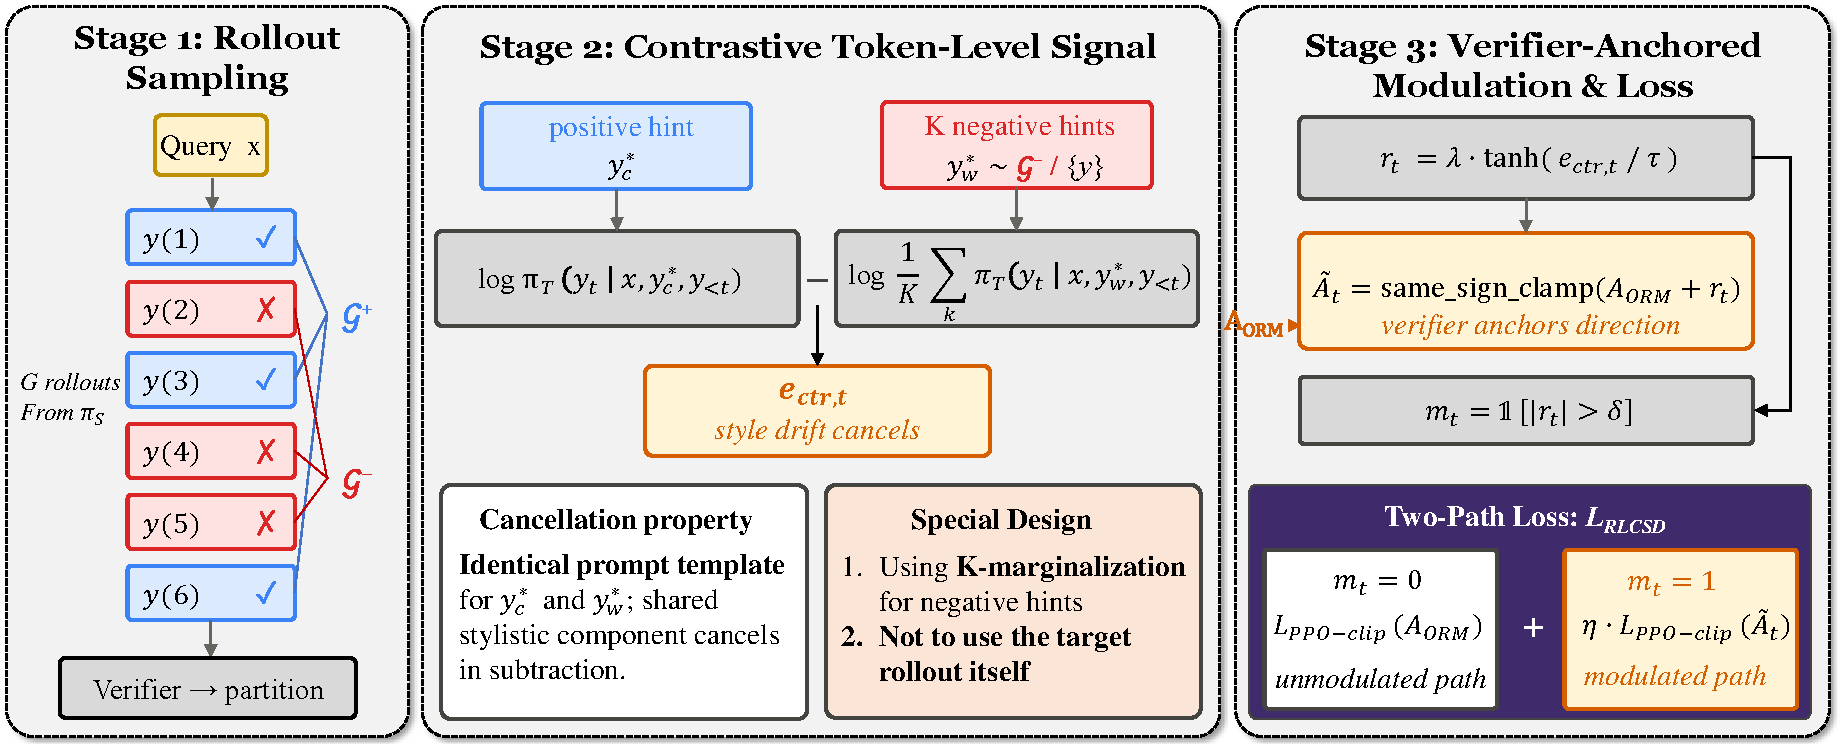
\includegraphics[width=\linewidth]{figs/RLCSD.pdf}
    \caption{Overview of \textbf{RLCSD}, illustrated with the self-rollout instantiation in which the positive hint is sampled from a correct rollout.
    RLCSD more generally allows the positive privileged context to come from
    other sources, such as a dataset-provided ground-truth reasoning trace.
    \textbf{Stage 1} samples a group of rollouts and partitions them by the
    verifier into correct ($\mathcal{G}^+$) and incorrect ($\mathcal{G}^-$)
    subsets. \textbf{Stage 2} feeds a positive hint and $K$ negative hints to the teacher under an identical template; their contrast yields the token-level signal $e_{\mathrm{ctr},t}$, in which the shared privilege-induced style component is substantially suppressed. \textbf{Stage 3} converts $e_{\mathrm{ctr},t}$ into a bounded modulation $r_t$, applies it to the verifier advantage $A_{\mathrm{ORM}}$ with a sign-preserving clamp, and aggregates a two-path clipped loss.}
    \label{fig:method-pipeline}
\end{figure}

Building on the diagnosis of privilege-induced style drift in Section~\ref{sec:drift}, RLCSD constructs a clean, token-level supervision signal by contrastive cancellation across symmetrically-formatted privileged contexts and uses it to modulate the verifier-derived advantage in a GRPO objective. Figure~\ref{fig:method-pipeline} illustrates the full pipeline, which consists of three stages:
\begin{itemize}
    \item \textbf{Stage 1: Rollout Sampling and Outcome Evaluation.}
    For each query, the model samples a group of rollouts, which are evaluated
    by the verifier. These rollouts provide the outcome-level GRPO advantage and are partitioned into correct and incorrect subsets, which serve as candidate pools for rollout-derived privileged contexts.
    \item \textbf{Stage 2: Constructing the Contrastive Token-Level Signal.}
    We pair a correct privileged context with a set of incorrect privileged
    contexts under an identical prompt template. The correct context can be
    obtained either from a successful student rollout or from a
    dataset-provided ground-truth reasoning trace, while the incorrect contexts are sampled from unsuccessful student rollouts.
    The contrastive difference between the positive and the negative branches yields a per-token signal $e_{\text{ctr},t}$ on sampled tokens in which the shared stylistic component is substantially reduced, leaving a signal that is more strongly tied to task correctness.
    Moreover, we introduce two design refinements, marginalizing over $K$ negative hints and excluding the current student rollout from any rollout-derived hint pool, both detailed in \S\ref{sec:method-ectr}.
    \item \textbf{Stage 3: Modulating the Outcome Advantage and Aggregating the Loss.} We convert $e_{\text{ctr},t}$ into a bounded per-token modulation $r_t$ and apply it to $A_{\text{ORM}}$ through clamping and masking, yielding a two-path PPO-style clipped aggregated loss~\citep{schulman2017proximal}.
\end{itemize}

The remainder of this section details each stage: privileged context construction (\S\ref{sec:method-hints}), construction of the contrastive token-level signal (\S\ref{sec:method-ectr}), verifier-anchored modulation of the advantage (\S\ref{sec:method-mod}), and the final two-path loss (\S\ref{sec:method-loss}).

\subsection{Constructing Privileged Contexts}
\label{sec:method-hints}

For each query $x$, we follow the GRPO sampling protocol and draw a group of $G$ rollouts $\{y^{(g)}\}_{g=1}^G$ from the student policy $\pi_S$. A rule-based verifier assigns each rollout a binary reward: $r=1$ if the extracted answer matches the ground truth and $r=0$ otherwise\footnote{All training tasks in our experiments use binary (0/1) rewards. For math tasks the verifier extracts the $\backslash$\texttt{boxed\{\}} answer and checks equivalence; for Knights-and-Knaves it parses the assignment list.}. This partitions the group into a correct subset $\mathcal{G}^+$ and an incorrect subset $\mathcal{G}^-$. Groups for which either subset is empty are discarded; this discards no useful training signal, because a uniform-outcome group already yields zero advantage under GRPO's group-relative normalization.

\paragraph{Symmetric prompt templates for positive and negative hints.}
For each non-discarded group, we pair a \emph{positive privileged context} $y_c^*$ with one or more \emph{negative privileged contexts} drawn from $\mathcal{G}^-$. The positive context can either be sampled from a correct student rollout in $\mathcal{G}^+$ or taken from a dataset-provided ground-truth reasoning trace. Each hint is wrapped in an identical prompt template consisting of (i) the original problem statement, (ii) the reference solution's full reasoning trace, (iii) its final answer, and (iv) a continuation instruction that transitions from the reference block to the teacher's own response. The template used in our main experiments is shown below. Critically, the template makes no distinction between correct and incorrect hints: a negative hint is presented with the same ``Reference Solution'' framing and ``Correct final answer'' label as a positive one, so the teacher treats both as ground-truth references and produces distributions that differ \emph{only} in what the reference says. Because the template is byte-for-byte identical across the two branches, the privilege-induced stylistic shift is more likely to be shared between them and therefore partially cancels in the subtraction $e_{\text{ctr},t}$, leaving the signal more task-bearing in practice.

\begin{tcolorbox}[
    colback=purple!5!white,
    colframe=richpurple!80!black,
    boxrule=1pt,
    arc=2mm,
    left=3mm, right=3mm, top=2mm, bottom=2mm,
    fonttitle=\bfseries,
    title=\textbf{Teacher Privileged Prompt Template}
]
\texttt{Problem: \{problem\}}\\[4pt]
\texttt{Here is a reference solution to this problem:}\\[4pt]
\texttt{\textcolor{teal}{=== Reference Solution Begin ===}}\\[4pt]
\texttt{\{reference solution text\}}\\[2pt]
\texttt{Correct final answer: \{extracted answer\}}\\[4pt]
\texttt{\textcolor{teal}{=== Reference Solution End ===}}\\[4pt]
\texttt{After reading the reference solution above, make sure you understand the reasoning behind each step.}
\texttt{Please reason step by step, and put your final answer within} $\backslash$\texttt{boxed\{\}}\texttt{.}
\end{tcolorbox}

\subsection{Contrastive Token-Level Signal}
\label{sec:method-ectr}

\paragraph{The vanilla form of $e_{\text{ctr},t}$.}
The most vanilla instantiation of the contrastive signal pairs a correct privileged context $y_c^*$ with a single incorrect privileged context $y_w^*$, and takes the difference of the two teacher--student log-probability gaps:
\begin{equation}
    e_{\text{ctr},t}^{\textcolor{naivered}{(\text{vanilla})}}
    = e_{c,t} - e_{w,t}
    = \log \pi_T(y_t \mid x, y_c^*, y_{<t})
    - \log \pi_T(y_t \mid x, y_w^*, y_{<t}),
\end{equation}
where $y_c^*$ is either a correct student rollout sampled from $\mathcal{G}^+$ or a dataset-provided ground-truth reasoning trace, while $y_w^*$ is sampled from the incorrect rollout subset $\mathcal{G}^-$.
This vanilla form suffers from two structural problems, which motivate two corresponding refinements.


\paragraph{Refinement 1: $K$-marginalized negative hints.}
A direct use of the vanilla contrast is unstable because incorrect solutions are highly heterogeneous: for an incorrect target rollout $y$, a randomly sampled negative hint $y_w^*$ may correspond to a very different error type, in which case the teacher conditioned on $y_w^*$ does not reliably endorse the tokens of $y$. The negative branch then ceases to provide a stable counter-signal, weakening the directional consistency of $e^{(\mathrm{vanilla})}_{\mathrm{ctr},t}$ and injecting noise into training. To address this, instead of conditioning on a single incorrect rollout, we sample $K$ negative hints independently from $G^-$ and average their probabilities in the negative branch. This replaces a brittle one-to-one contrast with a more stable estimate against the error distribution represented by the group. Empirical evidence is provided in Appendix~\ref{app:negative-hint}.

\begin{wrapfigure}{r}{0.42\linewidth}
  \centering
  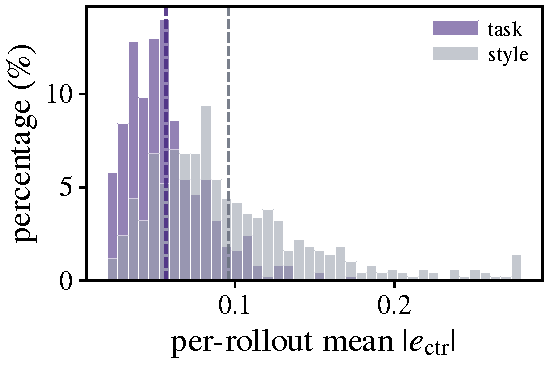
\includegraphics[width=\linewidth]{figs/hist_ectr_task_vs_style.pdf}
  \caption{Task/style analysis of $|e_{\mathrm{ctr},t}|$. The reduced style--task gap indicates a cleaner signal than $|e_c|$ (Figure~\ref{fig:ec-task-vs-style}).}
  \label{fig:ctr-clean}
  \vspace{-15pt}
\end{wrapfigure}

% \paragraph{Refinement 2: excluding the target rollout from the hint pool.}
% When a privileged context is drawn from the rollout group, the target rollout $y$ itself may be selected as its own hint. Conditioning the teacher on $y$ induces extreme over-confidence, making the signal overly sharp and obscuring the token-level distinctions that $e_{\text{ctr},t}$ is meant to capture. We therefore \textbf{exclude $y$ from all rollout-derived hint pools}: negative hints are drawn from $\mathcal{G}^-\setminus\{y\}$, and self-generated positive hints, when used, are drawn from $\mathcal{G}^+\setminus\{y\}$. Appendix~\ref{app:self-hint} quantifies the over-confidence effect that motivates this choice.

\paragraph{Refinement 2: excluding the target rollout from the hint pool.}
When a privileged context is drawn from the rollout group, the target rollout $y$ itself may inadvertently be selected as its own hint. In this case, the teacher is given the exact response whose token probabilities it is asked to evaluate. Conditioning on $y$ induces extreme over-confidence in its tokens, making the resulting signal overly sharp and obscuring the token-level distinctions that $e_{\text{ctr},t}$ is meant to capture. We therefore \textbf{exclude $y$ from all rollout-derived hint pools}: negative hints are drawn from $\mathcal{G}^-\setminus\{y\}$, and self-generated positive hints, when used, are drawn from $\mathcal{G}^+\setminus\{y\}$. This ensures that each rollout-derived hint is a separate trajectory rather than the target rollout itself. Appendix~\ref{app:self-hint} quantifies the over-confidence effect that motivates this choice.

\paragraph{Final $e_{\mathrm{ctr},t}$ and its effect.}
Combining the two refinements, the final contrastive signal is
\begin{equation}
\small
e_{\mathrm{ctr},t}
= \log \pi_T(y_t \mid x, y_c^*, y_{<t})
- \log \frac{1}{K}\sum_{k=1}^{K}
\pi_T(y_t \mid x, y_{w,k}^*, y_{<t}),
\quad
\{y_{w,k}^*\}_{k=1}^{K}
\sim \mathcal{G}^-\!\setminus\!\{y\}.
\label{eq:final-ectr}
\end{equation}
Here, $y_c^*$ denotes the correct privileged context: it is either sampled
from $\mathcal{G}^+\setminus\{y\}$ in the self-rollout instantiation or
taken directly from a dataset-provided ground-truth reasoning trace.
Since the shared template makes the privilege-induced style component more similar across the two branches, the subtraction suppresses this shared component, leaving the signal more task-bearing. Repeating the task/style analysis of Section~\ref{sec:drift} on
$|e_{\mathrm{ctr},t}|$ (Figure~\ref{fig:ctr-clean}) confirms this: the
style--task separation seen under $|e_c|$ (Figure~\ref{fig:ec-task-vs-style})
is substantially reduced, shifting weight onto the task-bearing tokens that
determine the answer.


\subsection{Verifier-Anchored Modulation of the Advantage}
\label{sec:method-mod}

\paragraph{Outcome-level GRPO advantage.}
For each query $x$, GRPO samples a group of $G$ rollouts
$\{y^{(g)}\}_{g=1}^{G}$ from the old policy $\pi_{\theta_{\text{old}}}$.
A verifier assigns each rollout an outcome reward
$R^{(g)} \in \{0,1\}$. The outcome-level advantage is then computed
by group-relative normalization:
\begin{equation}
\label{eq:aorm}
A_{\text{ORM}}^{(g)}
=
\frac{
R^{(g)} - \frac{1}{G}\sum_{j=1}^{G} R^{(j)}
}{
\sqrt{\frac{1}{G}\sum_{j=1}^{G}
\left(R^{(j)} - \frac{1}{G}\sum_{\ell=1}^{G} R^{(\ell)}\right)^2}
+ \epsilon_{\text{adv}}
}.
\end{equation}
This scalar advantage is broadcast to all tokens in rollout $y^{(g)}$.
Thus, $A_{\text{ORM}}^{(g)}$ provides a verifier-grounded trajectory-level
update direction, but it does not distinguish which intermediate tokens
are responsible for the final outcome.

Drawing on the ideas behind Xiaomi MiMo's OPD algorithm~\citep{xiao2026mimo} and RLSD~\citep{yang2026self}, we do not treat the teacher--student log-probability gap as the sole source of learning signal. Instead, we use the verifier-derived $A_{\text{ORM}}$ as the anchor that determines the update direction, and use the contrastive token-level signal $e_{\text{ctr},t}$ only to modulate its magnitude at selected tokens. The specific procedure is as follows.

\paragraph{Soft normalization and rescaling.}
Raw $e_{\text{ctr},t}$ values can be heavy-tailed, with occasional outlier tokens producing values that would dominate the optimization. We first squash them through a hyperbolic tangent and then rescale the result by a factor $\lambda$:
\begin{equation}
\label{eq:rt}
r_t = \lambda\tanh\!\left(\frac{e_{\text{ctr},t}}{\tau}\right) \in (-\lambda, \lambda),
\end{equation}
where $\tau$ controls the soft-threshold slope and $\lambda$ sets the overall scale.

\paragraph{Token-level mask.}
Many tokens carry an $r_t$ whose absolute value is very small; these can be regarded as noise. We therefore apply a token-level mask to single out the subset of tokens carrying contrastive signal strong enough to warrant modulation, and only these tokens have their advantage modulated by $r_t$:
\begin{equation}
\label{eq:mt}
m_t = \mathbb{1}(|r_t| > \delta).
\end{equation}
Empirically, $m_t = 1$ for roughly 20\% to 30\% of tokens, consistent with the observation that a small fraction of high-influence tokens determines the outcome of long reasoning chains.

\paragraph{Sign-preserving clamp.}
For the tokens selected for modulation, we add $r_t$ to the GRPO advantage $A_{\text{ORM}}$ broadcast to token $t$ and clamp the result so that it retains the sign of $A_{\text{ORM}}$:
\begin{equation}
\label{eq:samesign}
\tilde{A}_t =
\begin{cases}
\max(0, \, A_{\text{ORM}} + r_t) & \text{if } A_{\text{ORM}} \ge 0, \\
\min(0, \, A_{\text{ORM}} + r_t) & \text{if } A_{\text{ORM}} < 0.
\end{cases}
\end{equation}
This safeguard prevents the contrastive modulation from reversing the verifier-determined direction at any individual token.

\subsection{Two-Path Loss Aggregation}
\label{sec:method-loss}

We write the RLCSD optimization target as a PPO-style clipped surrogate
objective to be maximized; in implementation, we minimize its negative
as the training loss. The objective contains two paths: an unmodulated
path for tokens with $m_t=0$, which uses the original outcome-level
advantage $A_{\text{ORM}}$, and a modulated path for tokens with $m_t=1$,
which uses the sign-preserving modulated advantage $\tilde{A}_t$.

For rollout $y^{(g)}$, let
\begin{equation}
\rho_{g,t}(\theta)
=
\frac{
\pi_\theta(y^{(g)}_t \mid x, y^{(g)}_{<t})
}{
\pi_{\theta_{\text{old}}}(y^{(g)}_t \mid x, y^{(g)}_{<t})
}
\end{equation}
denote the per-token importance ratio. For a token with advantage $A$,
we define its clipped surrogate contribution as
\begin{equation}
\label{eq:clip-surrogate}
\psi_{g,t}(A; \theta)
=
\min\!\Big(
\rho_{g,t}(\theta) A,\;
\operatorname{clip}\!\big(\rho_{g,t}(\theta), 1-\epsilon, 1+\epsilon\big) A
\Big).
\end{equation}

For each rollout $y^{(g)}$, define the unmodulated and modulated token
sets as
\begin{equation}
\mathcal{U}^{(g)} = \{t : m^{(g)}_t = 0\},
\qquad
\mathcal{M}^{(g)} = \{t : m^{(g)}_t = 1\}.
\end{equation}
The rollout-level RLCSD surrogate objective averages the two paths
independently:
\begin{equation}
\label{eq:rlcsd-rollout-obj}
J_{\text{RLCSD}}^{(g)}(\theta)
=
\frac{1}{|\mathcal{U}^{(g)}|}
\sum_{t \in \mathcal{U}^{(g)}}
\psi_{g,t}\!\left(A_{\text{ORM}}^{(g)}; \theta\right)
+
\eta \cdot
\frac{1}{|\mathcal{M}^{(g)}|}
\sum_{t \in \mathcal{M}^{(g)}}
\psi_{g,t}\!\left(\tilde{A}^{(g)}_t; \theta\right),
\end{equation}
where $\eta$ controls the relative weight of the modulated path.
In the rare case that either token set is empty, the corresponding
path is omitted from the rollout-level objective.

Finally, the full query-level objective averages over the sampled group,
and the population objective averages over training queries:
\begin{equation}
\label{eq:rlcsd-full-obj}
J_{\text{RLCSD}}(\theta)
=
\mathbb{E}_{x \sim \mathcal{D}}
\left[
\frac{1}{G}
\sum_{g=1}^{G}
J_{\text{RLCSD}}^{(g)}(\theta)
\right].
\end{equation}
The training loss minimized in implementation is the negative of this
maximization objective:
\begin{equation}
\label{eq:rlcsd-loss}
\mathcal{L}_{\text{RLCSD}}(\theta)
=
- J_{\text{RLCSD}}(\theta).
\end{equation}

The choice to normalize the two paths independently within each rollout, rather than taking a single global mean over all tokens, is essential for preserving the influence of the contrastively modulated tokens. In practice, only about 20\%--30\% of tokens satisfy $m_t=1$; under a single global average, the modulated path would therefore contribute only in proportion to this small fraction and be easily overwhelmed by the unmodulated tokens. As a result, the token-level contrastive signal would be diluted, and the objective would drift toward plain GRPO, losing the fine-grained credit assignment that motivates RLCSD. Independent normalization avoids this dilution: it decouples the strength of the modulated path from the masked-token ratio $|\mathcal{M}^{(g)}|/|y^{(g)}|$, and makes $\eta$ the sole, explicit control over how much the contrastive signal contributes to training.

